\chapter{Case Study}\label{ch:case-study}

\section{Neverlang}\label{sec:neverlang}

Neverlang is a language workbench that allows the definition of new languages by composing existing languages. It is based on the idea of language-oriented programming, where the language is the main abstraction mechanism. Neverlang is implemented in Java and uses the dexter~\cite{Cazzola12d} parser generator to define the syntax of the languages. The semantics of the languages are defined using a combination of Java code and the Neverlang API. The Neverlang API provides a set of abstractions that allow the definition of language constructs, such as statements, expressions, and types. The API also provides mechanisms for defining the behavior of the constructs, such as how they are parsed, type-checked, and executed.

\subsection{The Neverlang type system}\label{sec:neverlang-type-system}

The type system in Neverlang is structured around various priorities that dictate the order of execution for tasks. These priorities are essential for maintaining the proper sequence and dependencies among different components of the language framework.

\subsubsection{Priorities}\label{sec:neverlang-priorities}

The priorities in Neverlang are used to determine the order in which different components of the language framework are processed. The priorities are defined as a set of constants in the \texttt{Priority} class, which is part of the Neverlang API. The priorities are used to ensure that the components are processed in the correct order and that all dependencies are satisfied.

\begin{enumerate}
    \item \textbf{Sources}: This priority is related to the root node, which is the starting point for the execution process.
    \item \textbf{Module}: After the root node, module declarations are executed. Modules form the fundamental building blocks and need to be processed early.
    \item \textbf{Syntax}: Syntax declarations are processed next, but they depend on module declarations because syntax can be imported from other modules.
    \item \textbf{Role}: Roles are linked to the symbols of a production, which means they depend on the syntax.
    \item \textbf{Slice}: Slices integrate roles and syntax, requiring the completion of both before they can be processed.
    \item \textbf{Bundle}: Bundles are collections of slices and modules, so they come after both.
    \item \textbf{Language}: The final priority is given to languages, which depend on the previously processed bundles and slices.
\end{enumerate}

\subsubsection{Types}\label{sec:neverlang-types}

The type system in Neverlang is based on the concept in which the types are used to represent the different constructs in the language framework. These types are categorized based on their functionality within the language framework.

\hfill \break
\noindent
\textbf{Language Features Related Types}:
\begin{itemize}
    \item \textbf{TypeBundle}: Represents a collection of slices and modules.
\item \textbf{TypeEndemicSlice}: A specific type of slice inherent to a particular context.
\item \textbf{TypeModule}: Represents a module within the language.
\item \textbf{TypeSlice}: Represents a slice that ties together roles and syntax.
\end{itemize}

\hfill \break
\noindent
\textbf{Internal Module Declaration Types}:
\begin{itemize}
\item \textbf{TypeCategory}: Defines categories within modules.
\item \textbf{TypeRole}: Represents roles within the module.
\item \textbf{TypeSyntax}: Represents syntax definitions within the module.
\end{itemize}

\hfill \break
\noindent
\textbf{Internal Syntax Declaration Types}:
\begin{itemize}
\item \textbf{TypeNonTerminal}: Non-terminal symbols in the syntax.
\item \textbf{TypeProduction}: Productions or rules in the syntax.
\item \textbf{TypeRegex}: Regular expressions used in the syntax.
\item \textbf{TypeTerminal}: Terminal symbols in the syntax.
\item \textbf{TypeLanguage}: Represents the overall language construct.
\end{itemize}

\subsection{Neverlang LSP}\label{subsec:neverlang-lsp}

The capabilities that have been implemented are:
\begin{itemize}
    \item Diagnostics
    \item Semantic Tokens
    \item Document Symbols
    \item References
    \item Go-to-definition
    \item Hover information
    \item Folding ranges
    \item Inlay hints
\end{itemize}

The ability to display symbols identifiers within productions is highly advantageous, as demonstrated in figure~\ref{fig:neverlang-lsp-before-after}. The annotations added beside each symbol serve as inlay hints, providing valuable visual cues to the user. The inlay hints are particularly useful for understanding the structure of the code and identifying the different components of the language constructs.

Workspaces are managed in a particular way, in fact the Language Server for each workspace tries to understand if the project is a gradle project:
\begin{itemize}
    \item if it’s a gradle project, all the projects listed in a Gradle file, which may include subprojects, are filtered to only include those with the "neverlang" pllugin. A workspace is created for each of these projects and then:
    \begin{itemize}
        \item The compilation classpath of the "neverlang" compiler is retrieved, and all classes that implement a "neverlang" unit are decompiled into "neverlang" source code.
        \item All the files in the "neverlang" source set, as well as any decompiled files, are analyzed.
    \end{itemize}
    \item if it’s not a gradle project, the Language Server is started for the workspace
\end{itemize}

\subsubsection{Some Implementation Details}\label{sec:neverlang-implementation-details}

In Neverlang, \textbf{terminal} and \textbf{non-terminal} symbols are treated in a special way. In the Listing~\ref{lst:type-production} the \texttt{TypeProduction} class is used to represent productions in Neverlang. The \texttt{TypeProduction} class has two counter, \texttt{terminalCounter} and \texttt{nonTerminalCounter}, which are used to keep track of the number of terminal and non-terminal symbols in the production. The \texttt{terminalCounter} and \texttt{nonTerminalCounter} are incremented whenever a terminal or non-terminal symbol is added to the production. The \texttt{terminalCounter} and \texttt{nonTerminalCounter} are used to determine the type of the production, which can be either a terminal production, a non-terminal production, or a mixed production.

\begin{Listing}
    \centering
    \showjava*[1\textwidth]{TypeProduction.java}
    \caption{TypeProduction class to represent productions in Neverlang}
    \label{lst:type-production}
\end{Listing}

\subsubsection{Different Ways to Referer to the Same Symbol}\label{sec:neverlang-different-ways-referer}

In Neverlang, there are different ways to refer to the same symbol. For example, we can use the position of the symbol in the production to refer to it, or we can use the alias of the symbol to refer to it. The alias of the symbol is a string that is used to refer to the symbol in the production. The alias of the symbol is set when the symbol is added to the production. The alias of the symbol is used to refer to the symbol in the production, and it is used to generate the symbol identifier for the symbol.

\begin{Listing}
    \centering
    \showneverlang*[1\textwidth]{ModuleProduction.nl}
    \caption{Module production in Neverlang}
    \label{lst:module-production}
\end{Listing}

Consider the code in Listing~\ref{lst:module-production}. There is the relative typelang code that performs the binding while, it can be noted that when there is no label associated with the production, the production type is bound to the "PRODUCTION" identifier, this identifier will be ignored in the binding phase in~\ref{lst:type-production}.

\subsubsection{Before and After LSP}\label{sec:neverlang-before-after-lsp}

Before the LSP generation, the source code of Neverlang in Visual Studio Code was not syntax-highlighted, and there was no support for go-to-definition or hover information etc. After the LSP generation, the source code of Neverlang in Visual Studio Code is syntax-highlighted, and there is support for go-to-definition, hover information, and other features provided by the LSP.

\begin{figure}[h!]
    \centering
    \begin{minipage}{0.45\textwidth}
        \centering
        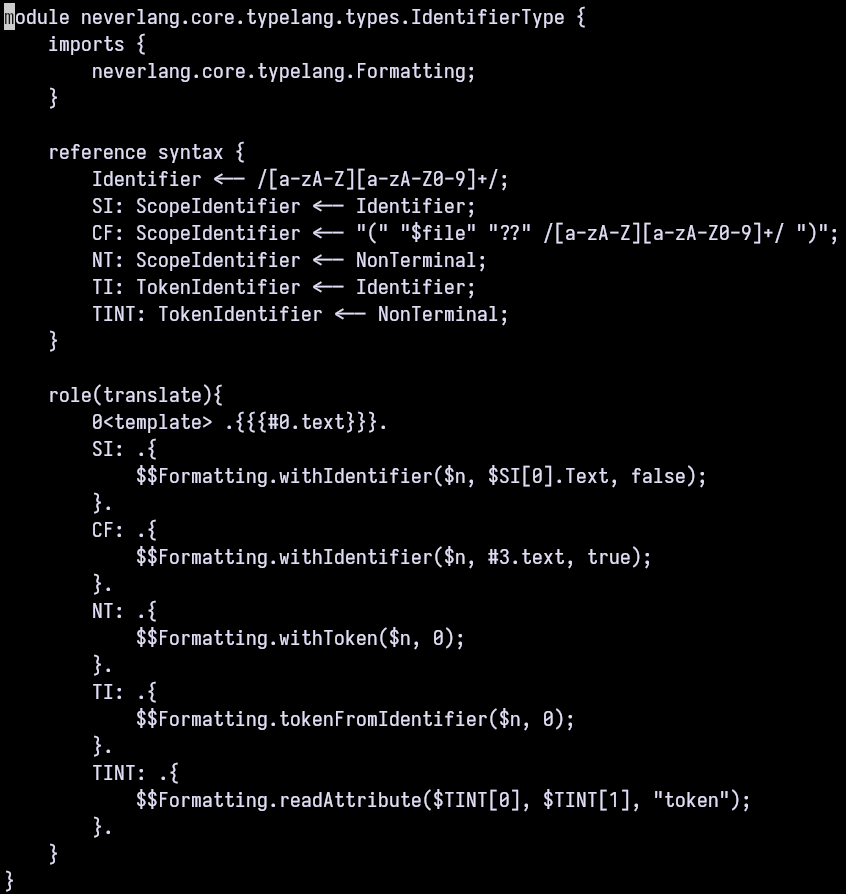
\includegraphics[width=\linewidth]{./imgs/neverlang-lsp-before-vim.png}
        \caption{Neverlang source code before the LSP generation}
    \end{minipage}\hfill
    \begin{minipage}{0.45\textwidth}
        \centering
        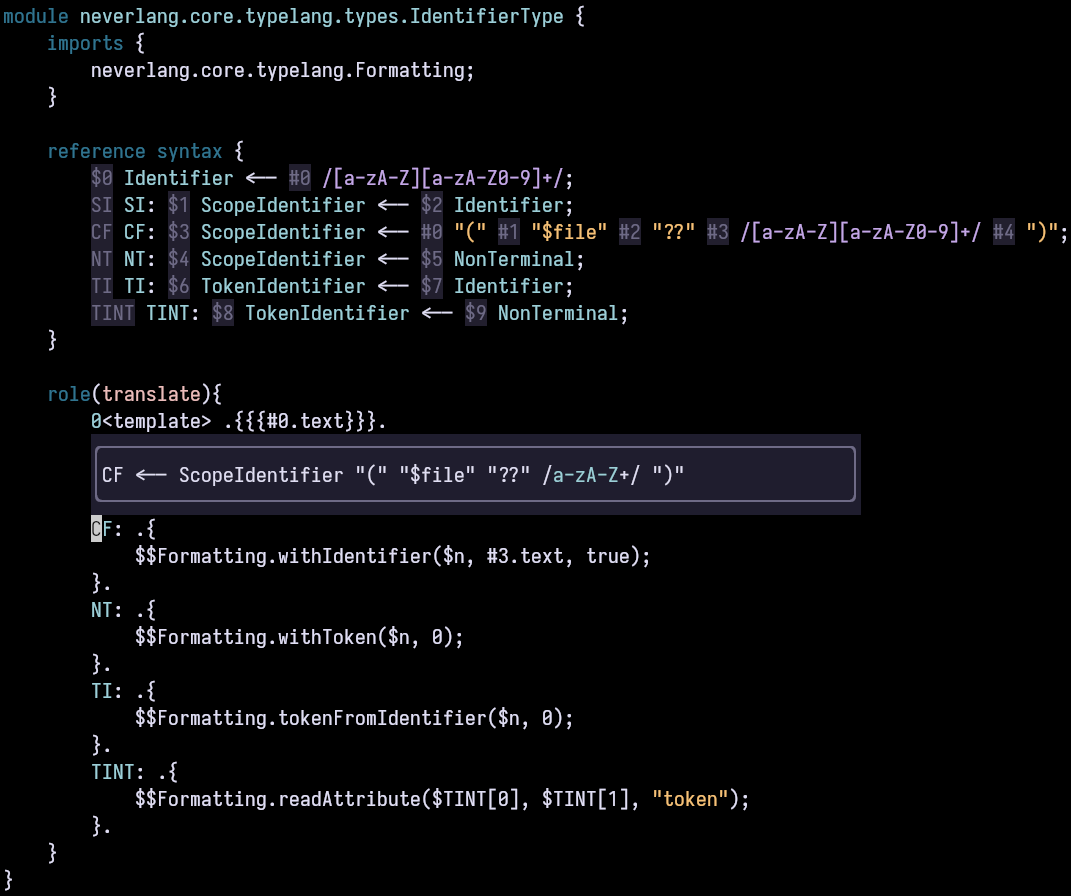
\includegraphics[width=\linewidth]{./imgs/neverlang-lsp-after-vim.png}
        \caption{Neverlang source code after the LSP generation}
    \end{minipage}
    \label{fig:neverlang-lsp-before-after}
\end{figure}



